
\documentclass[proposal]{softeng}

\usepackage{times,color}
\usepackage{hyperref, url}
\title{Generating Representative Artificial Datasets for Algorithm Evaluation}
\author{\ Dan-Florin Berbec \\ \ Supervisor: Peter Bloodsworth}
\organisation{University of Oxford}
\college{Kellogg College}
\award{Software Engineering} 


 \date{November 2019}
\usepackage[parfill]{parskip}
\usepackage{amsmath}
\begin{document}

\maketitle

\newpage
\clearpage\mbox{}\clearpage

\begin{abstract}
Proprietary complex algorithms are one of the main assets for many IT companies and their correctness is fundamental in fields such as finance and medicine, or simply when using an app that provides directions to a user or makes suggestions based on personal information. We may expect in the near future that some multi-million companies will reside mostly in the cloud with only a handful of employees. For regulators, investors or companies that have an interest in buying or investing in such a company, the task of validating the IP becomes difficult, especially when all that is accessible to a buyer is a black box with a limited amount of test data. We aim to assess the tools available to reliably and independently evaluate algorithms and present a process that can provide confidence to potential buyers that an algorithm works indeed as specified.\end{abstract}
 
\section{ Introduction}
\subsection{Area of study}

Algorithms are present in almost every electronic device we buy. From a simple light switch to running an OS and applications on a smartphone, their influence reaches beyond our daily decisions. For example, algorithms in a smartphone may direct a taxi driver on an alternative route based on congestion indicators set by a real-time data feed. Similarly, the prices of products in a supermarket may be influenced by low latency foreign exchange algorithms trading in an investment bank.

While simple algorithms have been around for many years aiding our decisions, complex ones now become ubiquitous in our decision-making process, many times with a significant outcome. Almost all industries including finance and healthcare or governmental institutions use algorithms to process large amounts of data to optimise spending resources. For example, a review\cite{algassessment} from the New Zealand government shows how crucial algorithms are in ensuring the wellbeing of the population. Ministries of justice, education and healthcare, customs and police, all use algorithms and data to improve their efficiency. Algorithms allow for data to be gathered and analyzed, identifying key areas where young people need support or helping to aggregate data and address risks at border control. Passport and visa applications can also be automated to reduce waiting times and allow staff to manually process the ones that reach a risk threshold. However, the review clearly states that significant decisions are still currently made by humans. 

Another example shows the US justice system relying much more heavily on algorithms - these are used to provide a likelihood score of a convict to re-offend and is one of the main factors for a judge when deciding a sentencing\cite{jail}. The algorithm used is trained on historical data and seems to have biases correlated to a convict financial status - it transforms these biases into causations. Importantly, the underlying algorithm is private and not made available to the public for assessment.

Finance also relies heavily on automation and algorithmic trading is rising very fast. Robot advisors are slowly replacing or at least aiding financial advisors to reduce the commissions charged as well as improve the performance of a fund\cite{robot}. For most financial institutions, especially large investment banks, regulators require backtesting to be executed and results sent for analysis\cite{backtesting}. This aims to ensure that trading strategies performing live today can also handle data in extreme environments such as the financial crisis in 2008.

While most of the algorithms used in decision making are currently crunching data to produce a deterministic output, newer types of algorithms within Machine Learning (ML) and Artificial Intelligence (AI) aim to train on historical data to find patterns that are applicable on new test data. From systems that recommend similar items to a virtual Go player that can beat a world champion\cite{alphago}, ML algorithms become increasingly trusted to performs functions that may significantly affect people's life. Huge investments are poured into self driving cars and a large number of big tech companies as well as many start ups\cite{autonomous} claim a share of this funding. These smart algorithms powering the cars may be expected to take the right decisions in noisy environments that have not been part of the training data, or ethical ones with no clear solutions, such as the trolley problem\cite{trolley}. As they are designed by humans, biases are also likely to influence the algorithm design.

One of the main assets of ML companies lies in developing such algorithms and preserving their secrecy. For big tech giants, such as Google, Uber or Waymo, theft of trade secrets is a serious concern and lawsuits are commonplace\cite{stealuber,waymo}. Algorithmic trade secrets, such as trading software, are also crucial in the financial industry, and any attempt for industrial espionage is thoroughly chased\cite{jeopardy}.

Provided that secrecy is of utmost importance for ML companies across all industries, many questions arise from stakeholders: how can regulators verify the fairness/lack of bias of a financial algorithms? Will an algorithmic robot trained on worst case scenario data from the 2008 financial crises perform as well during a new financial crises with different root causes? How can a judge have confidence that no bias is part of the score given to a convict if the underlying algorithm is only accessible to a handful of people? How can investors evaluate that the product of an ML company does indeed what is says it does?

Most of the time, a blackbox is provided to an external audit or potential investor with limited test data. Furthermore, this data could easily be proprietary as well and cleaned to fit the claims of the product. Currently, it seems that stakeholders do not have any means to independently verify that an algorithm does indeed what it says it does. 

With the increasing rise of tech startups, we may assume that in the near future, multi billion dollar companies may have only a handful of employees with a codebase living in the cloud and their main asset being IP. Their algorithms may have significant decisions for the public, yet understanding why a decision has been taken will be challenging to explain.



\subsection{Proposed work}

The aim of this project is to investigate the decision making process of auditing proprietary algorithms and propose methods to realistically improve the process. However, these general guidelines will aim to be applicable to any organisation independent of the size or industry.

Given the rise of machine learning algorithms and in particular deep learning, the project aims to primarily assess their explainability especially for cases where these are provided as a black box with a limited amount of proprietary test data. Deep learning mainly provides two types of algorithms: supervised and unsupervised learning. Supervised learning is used for classification purposes while unsupervised learning aims to find patterns within a data sets that are not mapped to specific labels.

One of the most commonly used supervised classification algorithm is powered by artificial neural networks (ANN). These are trained on test data sets and make predictions on new inputs. Their efficiency can be measured on how accurate their predictions are. For example, given a dataset of customers leaving a bank, a ANN can make future predictions based on independent variables on whether a customer is likely or not to leave the bank as well. A ANN could also decide based on income and age, whether a customer should be granted a loan or not. Another example could be a ANN making stock price predictions. While the algorithm is not public, it would be crucial for customers to have the ability to measure its performance before placing any money of their savings.

But ANN can easily be trained to perform well on some test data while new independent data would decrease their performance significantly or rendering the multi-million dollars algorithm worthless.

The scope of this project will mainly focus on assessing ANNs with a special interest in analyzing the training and test data available to evaluate the algorithm. We will look whether statistical inferences can be derived from the provided data and tools to expand or generate new data with similar parameters. The aim is also to test the behaviour of the algorithm under worst case scenarios or perform other modifications to the dataset to identify potential poor performance that impacts the validity of testing and its efficiency. This may include discussing big data architectures, working out patterns in data, generating random numeric datasets or creating altered datasets to test extremes. Unsupervised deep learning algorithms such as self organising maps could provide great help. Blackbox testing strategies applicable to deep learning will also be investigated. 

Provided that one of the main focuses of the dissertation will be on analysing the visible test data, we may argue that the underlying algorithm within the black box is not relevant. However, each algorithm requires a specific format for the data to be provided in. Thus, understanding the underlying algorithms and being able to modify these is just as important as the dataset analysis: it will provide a deeper understanding of potential issues from the perspective of IP owner and help understand the accuracy of the algorithm performance.

The project will focus on the investigation of ANN test data, which is mostly numeric and human readable. As a stretch goal, it will be useful to apply any findings to test other types of supervised learning such as convolutional neural networks used for example to classify images, or recurrent neural networks which make predictions based on time series, for example the stock price of a company. Another stretch goal would also consider analysing reinforcement learning algorithms in a black box and comparing these with evaluation of deep learning ones. Can the steps used to evaluate a deep learning algorithm also be applied to evaluate a reinforcement learning algorithm? However, this project does not intend to analyse all the validity of test data for each type of supervised deep learning algorithm: it will strictly commit to analysing ANNs and depending on the time and relevance, extend the scope to convolutional and recurrent NN as stretch goals only.

The project will evaluate a number of open source ANNs used in a variety of fields such as healthcare, finance, or law. The algorithms may be packaged as runnable code with training and test data or as a black box with test data only. Using proprietary algorithms will be avoided where possible, but may be used if the case study provides useful information. 

The expected outcome will present the reader with a with a process to validate a company IP by using a set of tools and techniques such as statistical analysis, big data, applicability of generative adversarial networks, and preparation of test data to validate the algorithm.  These examples do not represent a commitment but rather a sample of what might be useful in developing the process, which  is subject to further background literature and the rapid growth of new ideas being published in the field. New solutions may be developed if the literature lacks answers to some of the problems presented, but only within the realistic timeline and scope of this project.


\subsection{Artificial Neural Networks}

Artificial Neural Networks have become very popular in recent years for creating Artificial Intelligence algorithms. The aim is to teach a machine how to extract and learn features of a data set to make new predictions by replicating processes happening in the biological brain. Using a simplified neural representation: the dendrites, nucleus and axon of a neuron are respectively abstracted for a theoretical algorithm as the input, processing node, and output. 

The ANN is build using visible input nodes (data you can see - ex. age, address, education, job status) that feed into several hidden layers of neural nodes further feeding into output nods, the visible binary or categorical output (ex loan application granted or declined) -see fig \ref{fig:simplenetwork}. A node in any layer can be connected to one or many  nodes in the next layer. Due to the complexity of the connections in the middle layers and the fact that the data is not easily readable, the middle layers are called hidden layers.

\begin{figure}[h!]
\centering
  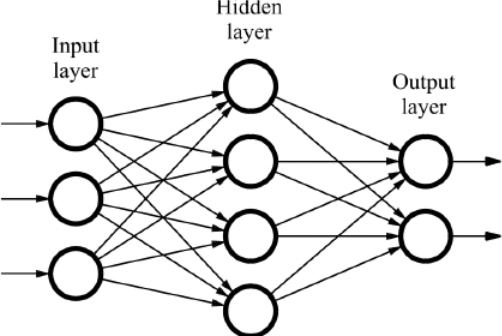
\includegraphics[scale=0.4]{images/simple-neural-network.jpg}
  \caption{Simple neural network with one hidden layer\cite{simpleneural}}
  \label{fig:simplenetwork}
\end{figure}

Each neuron in the network receives input from other nodes and computes this into a single output that feeds into other neurons or output nodes. A simple approach for a prediction could be to multiply an adjustable weight to each incoming input. To avoid producing zero values for zero inputs a bias can be added further as shown in eq  \ref{neuron}

\begin{equation}
\label{neuron}
 \sum_{i=1}^{n} {x_{i}} {w_{i}} + {b_{i}}  
\end{equation}
When the input \( {x_{i}} {w_{i}} \) is significantly less than the bias \({b_{i}}\) this implies that input has little effect. But over the training period the weight will be adjusted accordingly to overcome the effect of the bias. The final sum is not bounded and thus can be largely different than the output of other nodes. Activation functions are used to contain this value between a specific range, most commonly between -1 or 0 and 1. For example, a simple activation function, binary step, solve this issue. But this cutoff function however will miss many small details and may only be used in binary classification problems. While there are many activation functions available, the most commonly used alternatives are the \textit{sigmoid} function and \textit{rectified linear unit} (ReLu)

\begin{equation*}
    f(n) = \begin{cases}
               0               & n = 0\\
               1               & n = 1\\
               f(n-1) + f(n-2) & \text{otherwise}
           \end{cases}
\end{equation*}


In multiclass classification problems, the output layer will have one neuron per class. The categories may or may not be mutually exclusive and a common way to pick the best prediction is to choose the one with the highest probability when using for example a sigmoid function. As neurons in the last hidden layer are not interconnected these probabilities are independent and need to be normalized to equal to 1. A simply function such as \textit{softmax} divides each probability but the total sum. When categories are non exclusive, a probability threshold for each output neuron such as 0.5 can be used to pick the final outcome.


final output layer with one neuron per class
one hot encoding
softmax activatoin function 

The ANN can be trained using an existing dataset of examples to make future predictions and the weights of each neuron are adjusted depending on the performance of the prediction vs the actual value. 




While this idea was mentioned as early as 1970   


















\newpage
\footnotesize

\bibliographystyle{plain}
\bibliography{template}

\clearpage


\end{document}
